%----------------------------------------------------------------------------------------
%	ANALISI DEI REQUISITI
%----------------------------------------------------------------------------------------

\section{Analisi dei requisiti}

%In questa sezione esporre brevemente i requisiti a cui il sistema proposto deve rispondere, concentrando l'attenzione sugli aspetti più rilevanti e facendo eventualmente uso di opportuni diagrammi di alto livello.\\

%  3 componenti & 8000 & 10000 \\

Riportiamo prima in prosa i requisiti utente completi, derivanti da alcune sessioni di 
knowledge crunching con il nostro partner che rappresenta l'esperto di dominio.
Successivamente riportiamo un analisi tecnica preliminare del sistema con
i requisti di sistema a punti. 

\subsection{Requisiti utente}

Il gestore di un hotel, l'albergatore, può supportare il sistema Ecotrip
installando la centralina in una o più camere. Una centralina comprende diversi
sensori cablati che andranno opportunamente sistemati all'interno della camera.
I sensori previsti per il primo prototipo di Ecotrip sono:

\begin{itemize}
    \item 1 sensore per rilevare il consumo elettrico
    \item 1 flussometro per misurare il consumo d'acqua fredda + 1 per l'acqua calda
    \item 1 termometro per misurare la temperatura dell'acqua fredda + 1 per l'acqua calda
    \item 1 sensore di luminosità per ogni finestra, per rilevare se la tenda è aperta o chiusa
    \item 1 sensore di temperatura ambientale
    \item 1 sensore di umidità ambientale
\end{itemize}

La centralina comprende anche un insieme di sensori per identificare se l'ospite
è presente nella camera o meno: questo specifico aspetto viene lasciato per
sviluppi successivi al primo prototipo, il quale "rileverà" la presenza
dell'ospite attraverso un semplice interruttore meccanico. Nel prodotto finale
prevediamo invece due possibilità:
\begin{itemize}
    \item nel caso in cui la camera dispone già di una centralina che accende e spegne
    l'impianto elettrico in base all'inserimento della chiave da parte
    dell'ospite, allora la nostra centralina identificherà la presenza in base
    all'attivazione degli impianti.
    \item negli altri casi doteremo la camera di un sensore per identificare se la porta
    di accesso è aperta/chiusa e di uno o più sensori di presenza da installare a
    soffitto, in modo da stabilire se l'ospite è entrato o uscito ogni volta che
    la porta viene chiusa.
\end{itemize}

Una volta installata, la centralina viene connessa alla rete wifi dell'hotel in
modo da consentirle l'accesso ad Internet, inoltre viene configurata abbinandola
al numero di camera. Dopo la configurazione, la centralina campionerà ogni X
secondi i dati da tutti i sensori e li invierà sul cloud: deve essere possibile
stabilire l'origine dei dati nei termini di hotel e camera. Infine il sistema
deve prevedere meccanismi di controllo dello stato (centralina online/offline) e
di manutenzione da remoto.

Gli amministratori di Ecotrip tramite un pannello di controllo web possono
gestire la lista degli hotel, le loro camere, visualizzare lo stato delle
centraline installate ed infine registrare l'account dell'albergatore.

L'albergatore potrà quindi accedere al pannello di controllo e, per ciascuna
delle sue camere, visualizzare i dati istantanei raccolti dai sensori ed
indicare i momenti di check-in e check-out di un ospite: quest'ultima funzione
manuale, in ottica di sviluppo futuro, sarà automatizzabile con la connessione
del pannello di controllo al gestionale dell'albergo.

Per ogni soggiorno, cioè il periodo tra il check-in ed il check-out dell'ospite,
saranno visualizzabili oltre che i dati sintetizzati, anche il consumo totale di
CO2 ed il punteggio "sostenibilità" ottenuto. Il calcolo della CO2 viene fatto
considerando il consumo elettrico utilizzato per alimentare la stanza, compreso
quello per il suo riscaldamentoe e quello stimato per riscaldare l'acqua: si
considera infatti che negli USA le camere vengono riscaldate unicamente con
pompa di calore e non si utilizza gas/metano. Per effettuare il calcolo CO2 deve
essere specificato per ciascun hotel il costo dell'energia nei termini di
CO2/Kilowatt. Il punteggio "sostenibilità" tiene conto, non solo della CO2
totale, ma anche del comportamento tenuto dall'ospite durante la sua permanenza.
Alcuni comportamenti penalizzanti sono:

\begin{itemize}
    \item il fatto di uscire dalla camera lasciando in periodo estivo di giorno tende aperte e condizionatore acceso a pieno regime.
    \item usare eccessiva acqua
\end{itemize}

L'ospite attraverso l'app Ecotrip può visualizzare i dati del suo soggiorno
corrente e di quelli passati, comprendenti sia i dati sintetizzati, che il
consumo CO2 ed il punteggio "sostenibilità" aggiornati in tempo reale.

Al fine di permettere all'ospite di collegarsi facilmente ed autonomamente ai
dati del proprio soggiorno, a quest'ultimo viene associato un token univoco,
contenente un codice casuale generato al momento del check-in, ed inviato alla
centralina della relativa camera. Alla centralina è collegato un transponder NFC
che deve essere installato nella camera in modo che sia visibile agli ospiti,
magari identificabile con il logo di Ecotrip. Quando un ospite avvicina al
transponder della centralina il proprio smartphone provvisto di NFC, questo
riceve indicazioni per avviare automaticamente l'app Ecotrip con il token come
parametro: da questo momento l'app memorizzerà il token e permetterà di
visualizzare i dati del soggiorno richiedendoli ad un servizio remoto.
L'operazione di collegamento token-app può essere fatta una sola volta e solo
prima del check-out, questo garantisce sicurezza e privacy riducendo il rischio
di violazioni di accesso ai dati.

Al check-out è possibile calcolare uno sconto in base alla CO2 risparmiata
rispetto a valori obiettivo e/o in base al punteggio "sostenibilità" ottenuto.

\subsection{Casi d'uso}
Presentatiamo i casi d'uso principali suddivisi per contesto (pannello di controllo, app e centralina) ed 
identificati a partire dai requisiti utente di cui sopra. 

\begin{figure}[H]
    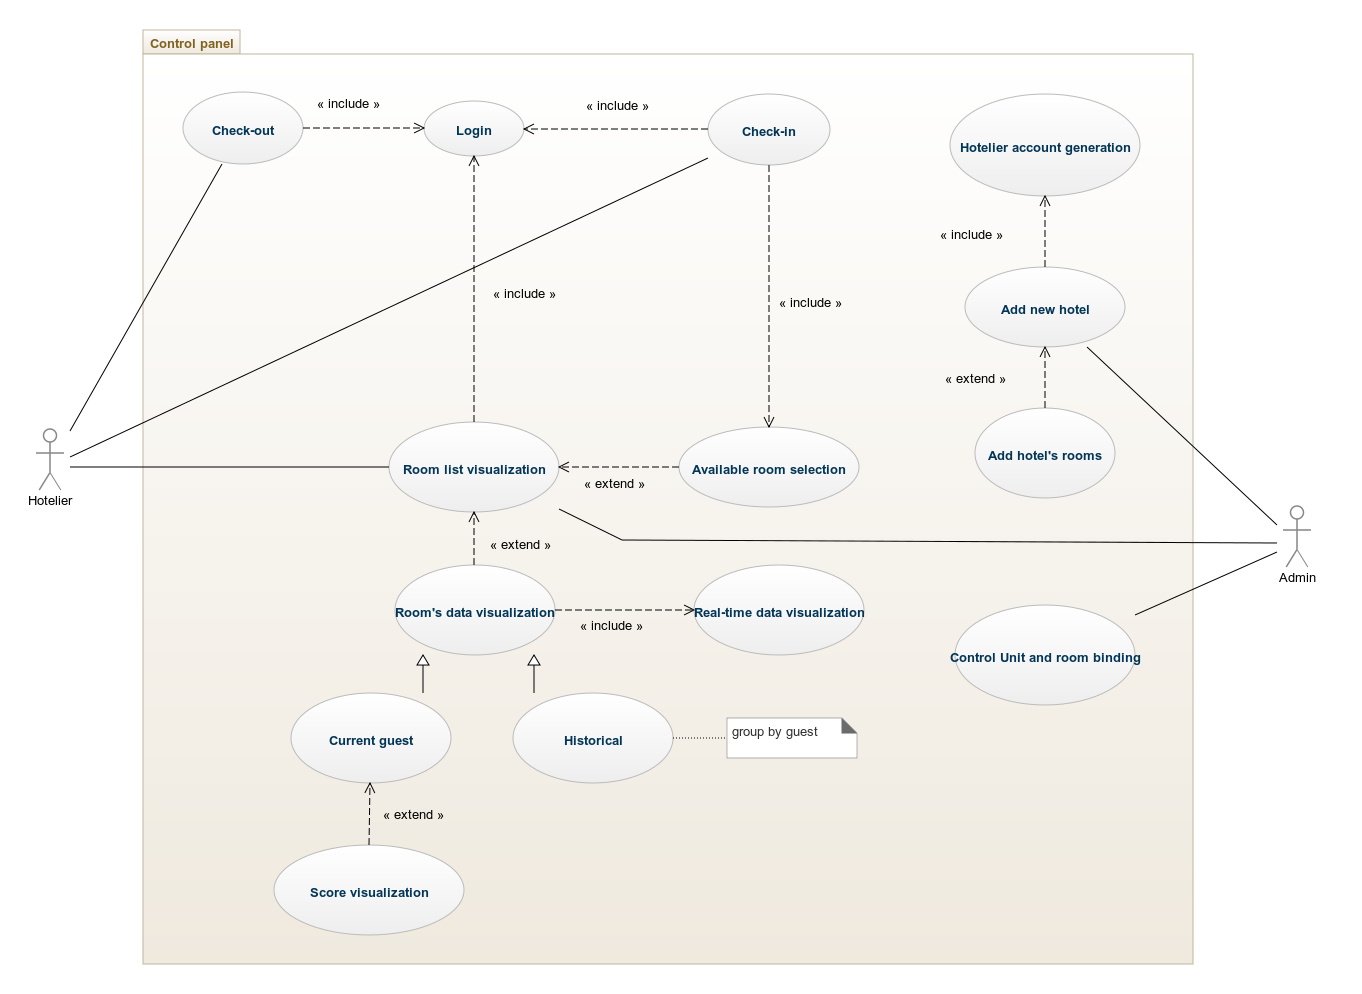
\includegraphics[width=\textwidth]{control-panel-usecase.png}
    \centering
    \caption[control-panel-usecase]{Schema dei casi d'uso del pannello di controllo.}
    \label{fig:cp-usecase}
\end{figure}

\begin{figure}[H]
    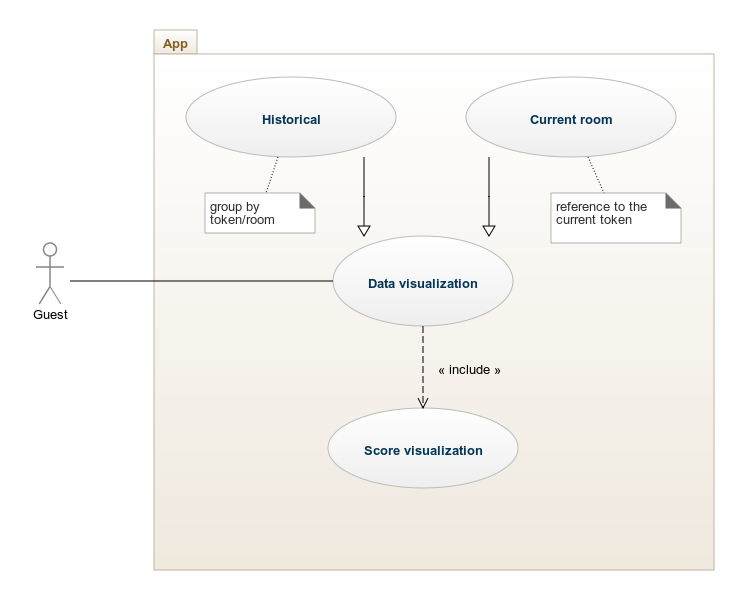
\includegraphics[width=0.8\textwidth]{app-use-case.png}
    \centering
    \caption[app-usecase]{Schema dei casi d'uso relativi all'applicazione lato ospite.}
    \label{fig:app-usecase}
\end{figure}

\begin{figure}[H]
    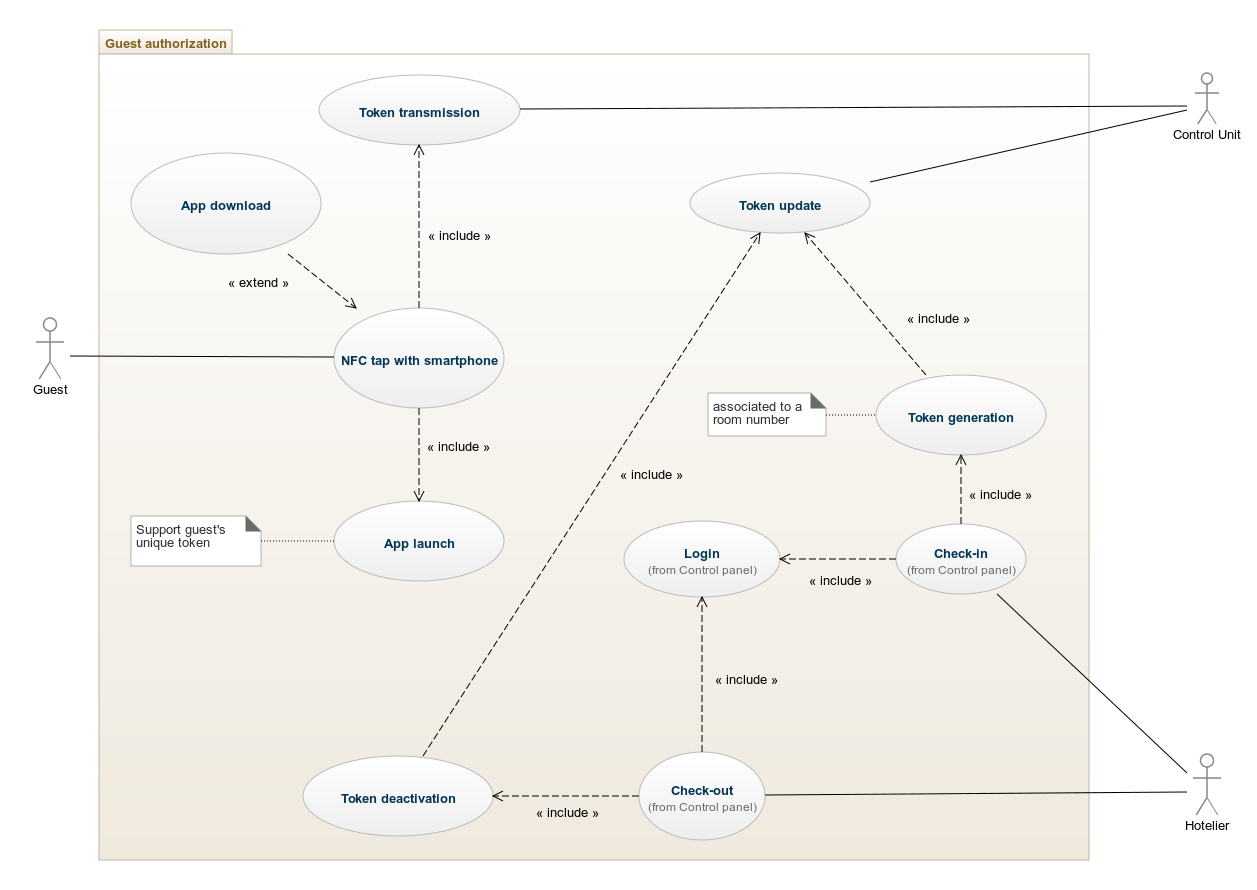
\includegraphics[width=\textwidth]{guest-authorization-use-case.png}
    \centering
    \caption[guest-authorization-usecase]{Schema dei casi d'uso del meccanismo di autorizzazione dell'ospite.}
    \label{fig:guest-authorization-usecase}
\end{figure}

\begin{figure}[H]
    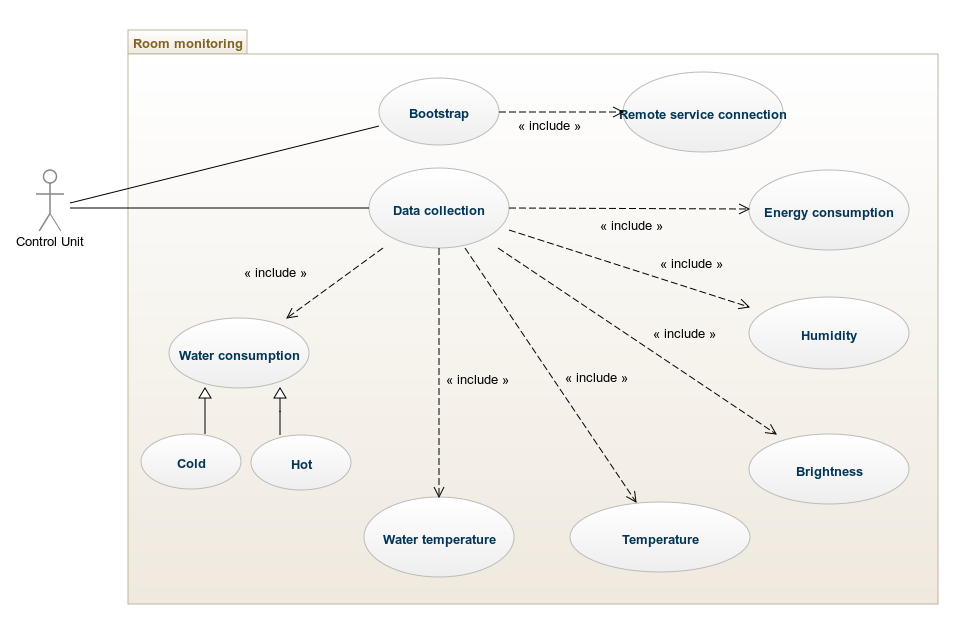
\includegraphics[width=\textwidth]{room-monitoring-use-case.png}
    \centering
    \caption[room-monitoring-usecase]{Schema dei casi d'uso relativi alla \textit{control unit}.}
    \label{fig:room-monitoring-usecase}
\end{figure}

\subsection{Sottodomini del problema}
Decomponiamo il nostro problema in 9 sottodomini (Figura \ref*{fig:subdomains}).
Un sottodominio (o un piccolo gruppo di questi) rappresenta un sotto-progetto indipendente con i propri requisiti, design e ciclo di sviluppo.

\begin{figure}[H]
    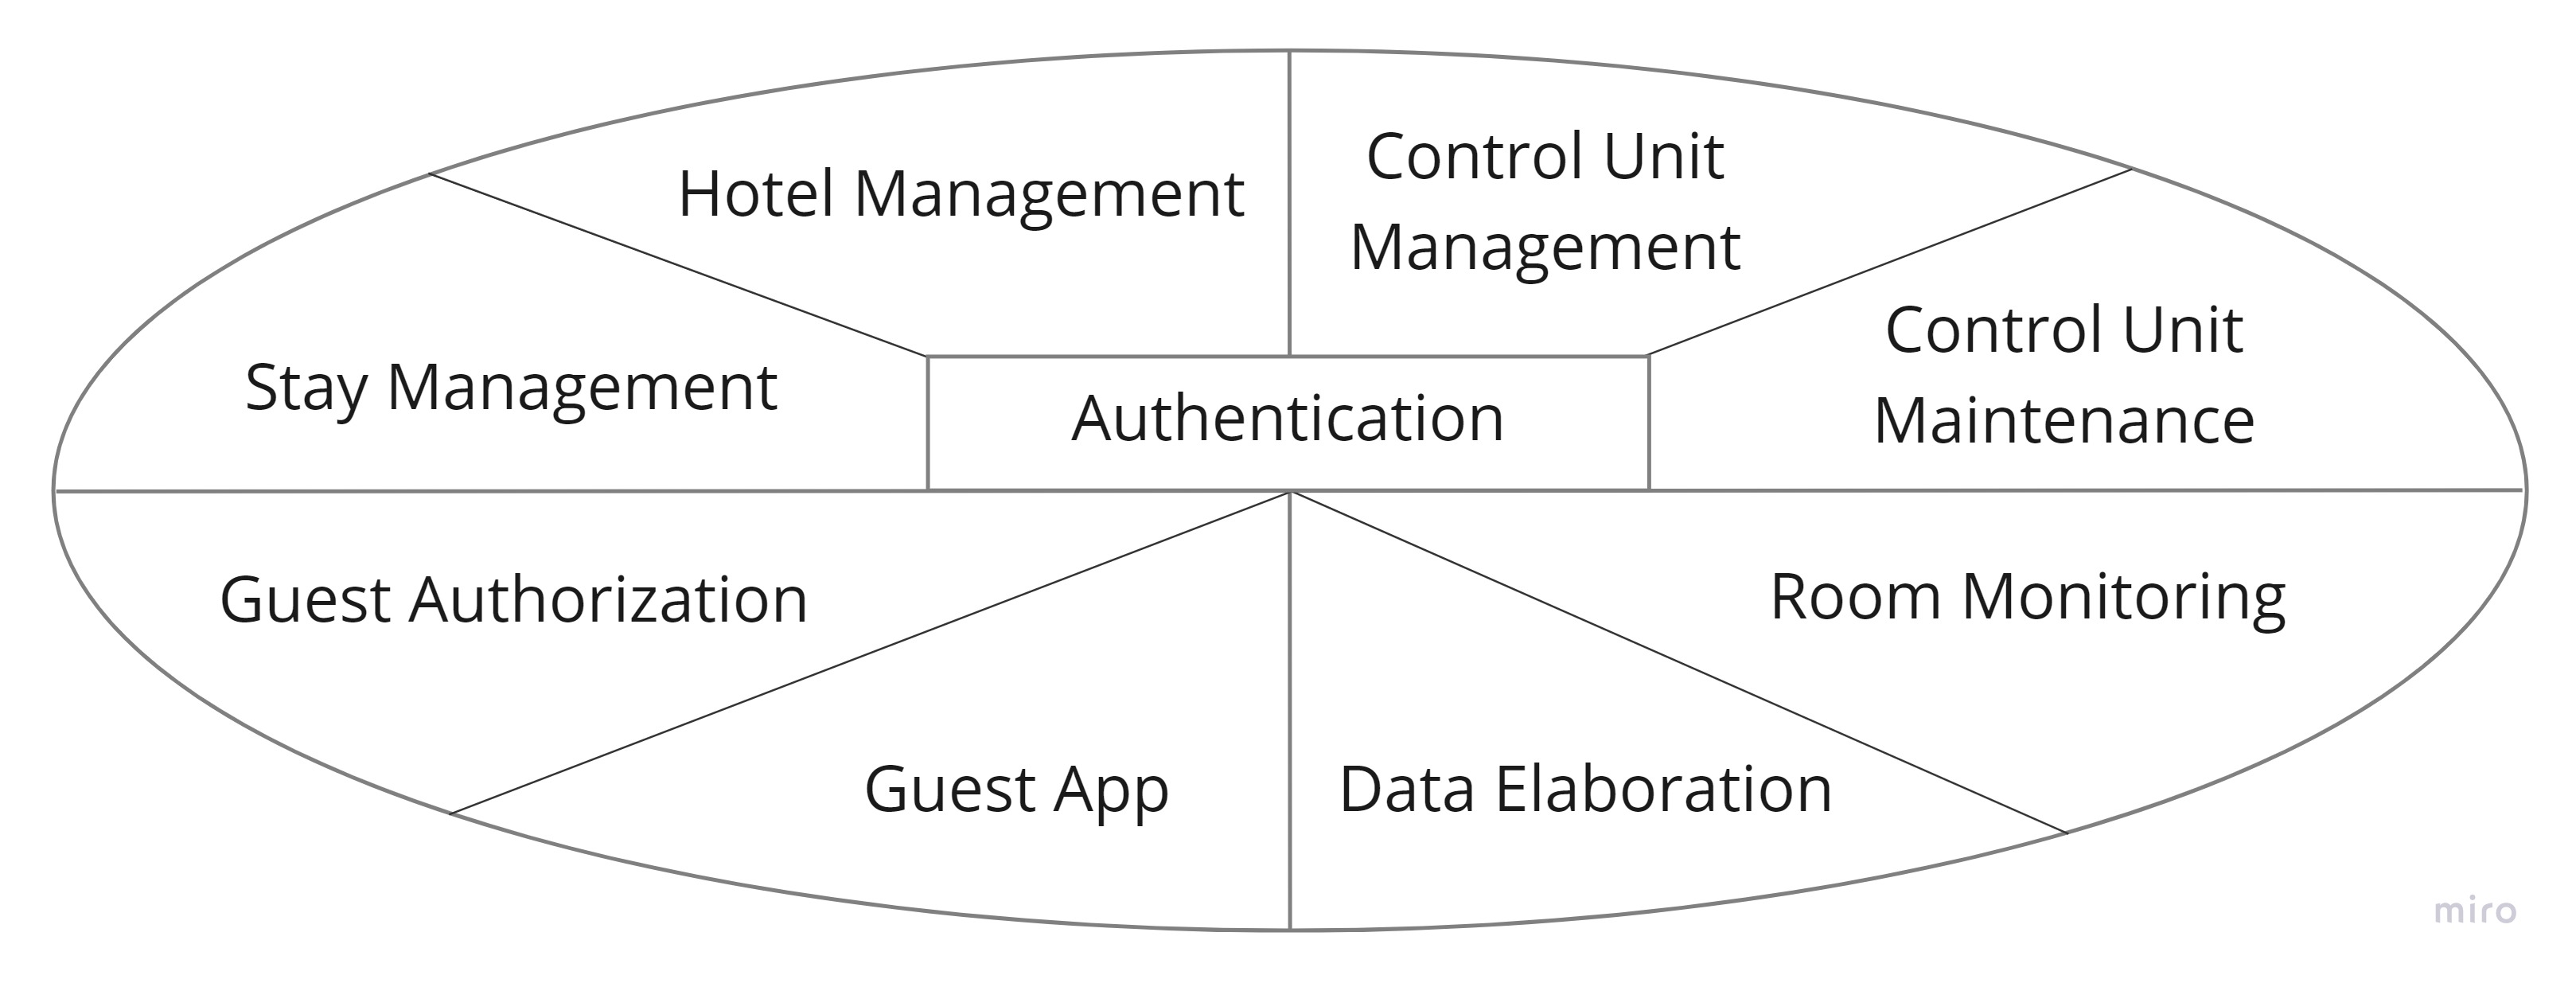
\includegraphics[width=\textwidth]{subdomains.jpg}
    \centering
    \caption[subdomains]{Sottodomini del sistema Ecotrip.}
    \label{fig:subdomains}
\end{figure}
\begin{itemize}
    \item \textit{Hotel Management}: comprende le funzionalità svolte dall'amministratore Ecotrip che riguardano la configurazione di nuovi hotel e relative camere.
    \item \textit{Stay Management}: comprende la gestione dei soggiorni con le funzioni di \textit{check-in} e \textit{check-out} da parte dell'hotelier.
    \item \textit{Authentication}: comprende sia l'autenticazione utenti quali amministratore Ecotrip e \textit{hotelier} richiesta per l'utilizzo dei servizi come \textit{Hotel} e \textit{Stay Management}, che la possibilità di registrare gli \textit{account} per gli \textit{hotelier}.
    \item \textit{Control Unit Management}: comprende la gestione delle centraline installate con la possibilità di verifica dello stato e di abbinamento alle camere.
    \item \textit{Control Unit Maintenance}: comprende il sistema per la manutenzione da remoto delle centraline installate.
    \item \textit{Room Monitoring}: comprende il sistema per il campionamento dei dati dai sensori della centralina e lo stoccaggio in un servizio cloud.
    \item \textit{Data Elaboration}: comprende il sistema per il calcolo della stima dei consumi C02 e del punteggio "sostenibilità" relativo ai soggiorni, a partire dai dati collezionati.
    \item \textit{Guest Authorization}: include il processo di generazione del \textit{token} per un nuovo soggiorno ed il suo trasferimento alla centralina e successivamente allo smartphone mediante \textit{transponder} NFC, permettendo così all'ospite di accedere ai dati del suo soggiorno.
    \item \textit{Guest App}: include la visualizzazione dei dati del soggiorno tramite applicativo fruibile dagli ospiti, inoltre implementa gli aspetti di \textit{gamification}.
\end{itemize}

\subsection{Requisiti di sistema}

Dettagliamo di seguito i requisiti di sistema funzionali suddivisi per i diversi sottodomini del sistema Ecotrip.
Successivamente specifichiamo i requisiti non funzionali.

\begin{itemize}
    \item Requisiti funzionali

    \begin{itemize}
        \item Authentication
        \begin{itemize}
            \item Autenticazione utenti con email e password
            \item Registrazione nuovi utenti
            \item Ruoli previsti: amministratori ecotrip e albergatori
        \end{itemize}
    \end{itemize}

    \begin{itemize}
        \item Room Monitoring
        \begin{itemize}
            \item Raccolta dati con campionamento ogni secondo da diversi sensori
            \begin{itemize}
                \item Rilevazione del consumo energetico con sensore di corrente
                \item Rilevazione del consumo di acqua tramite due flussometri
                \item Rilevazione della temperatura di acqua calda / fredda tramite due sensori di temperatura
                \item Rilevazione dello stato delle tende (aperte/chiuse) della stanza attraverso un sensore di luminosità installato su ogni finestra
                \item Rilevazione della temperatura della stanza mediante un sensore di temperatura ambientale
                \item Rilevazione della percentuale di umidità della stanza tramite un sensore di umidità ambientale
            \end{itemize}
            \item Identificazione presenza ospite all'interno della stanza (opzionale)
            \item Aggregazione dati campionati ogni 5 secondi
            \begin{itemize}
                \item Calcolo del consumo energetico
                \item Calcolo del consumo di acqua
            \end{itemize}
            \item Invio ogni 5 secondi dei dati rilevati ed aggregati a piattaforma cloud
        \end{itemize}
    \end{itemize}

    \begin{itemize}
        \item Guest Authorization
        \begin{itemize}
            \item Generazione token univoco, firmato e verificabile al checkin dell'ospite contenete identificativi di hotel, stanza e pernottamento
            \item Sincronizzazione su centralina del token generato in remoto
            \item Controllo sensore NFC su centralina per trasferire il token a dispotivo mobile
            \item Il tag NFC deve funzionare in modo da avviare sullo smartphone la web app Ecotrip senza azione dell'utente, 
                    ma solo all'avvicinamento del dispositivo al tag
        \end{itemize}
    \end{itemize}

    \begin{itemize}
        \item Control Unit Management
        \begin{itemize}
            \item Configurazione da parte degli amministratori Ecotrip di nuove centraline installate assegnando identificativo di hotel e stanza
            \item Verifica dello stato di funzionamento da remoto da parte degli amministratori Ecotrip
        \end{itemize}
    \end{itemize}

    \begin{itemize}
        \item Control Unit Maintenance
        \begin{itemize}
            \item Accesso da remoto a centralina installata da parte agli amministratori Ecotrip
            \item Aggiornamento automatico del software della centralina
        \end{itemize}
    \end{itemize}

    \begin{itemize}
        \item Hotel Management
        \begin{itemize}
            \item Accesso a pannello di controllo riservato solo agli amministratori ecotrip
            \item Gestione completa degli hotel con informazioni quali: identificativo, nome, indirizzo e costo dell'energia nei termini di CO2/Kilowatt
            \item Possibilità di creare l'account dell'albergatore per un hotel
            \item Gestione completa delle camere di un'hotel con informazioni quali: identificativo e numero
        \end{itemize}
    \end{itemize}

    \begin{itemize}
        \item Stay Management
        \begin{itemize}
            \item Accesso a pannello di controllo riservato agli amministratori ecotrip ed all'albergatore proprietario dell'hotel
            \item Visualizzazione dei pernottamenti suddivisi per camera
            \item Per ogni camera possibilità di eseguire check-in e check-out di un ospite
            \item Visualizzazione del punteggio "sostenibilità" del pernottamento con relativo consumo totale di CO2
            \item Visualizzazione dei consumi istantanei di una camera
        \end{itemize}
    \end{itemize}

    \begin{itemize}
        \item Data Elaboration
        \begin{itemize}
            \item Calcolo della CO2 a partire dai dati di un pernottamento
            \item Algoritmo per il calcolo del punteggio "sostenibilità" di un pernottamento a partire dalla CO2 generata e considerando il comportamento tenuto dall'ospite:
            \begin{itemize}
                \item uso eccessivo di acqua
                \item uscire dalla camera lasciando il condizionatore accesso e le tende aperte di giorno  
            \end{itemize}
        \end{itemize}
    \end{itemize}

    \begin{itemize}
        \item Guest App
        \begin{itemize}
            \item Avvio automatico con avvicinamento del dispositivo mobile al tag NFC
            \item Visualizzazione dei dati del pernottamento corrente: informazioni generali, consumo CO2 e "punteggio sostenibilità"
            \item Visualizzazione dei dati dei pernottamenti passati
        \end{itemize}
    \end{itemize}
    
    \item Requisiti non funzionali
    \begin{itemize}
        \item Garantire privacy per gli ospiti sia per quanto riguarda la scelta dei meccanismi/sensori utilizzati dalla centralina, 
                sia per quanto concerne la possibilità che qualcuno possa accedere ai dati non propri (esempio ospiti che accedono a dati di altri ospiti)
        \item Scalabilità del sistema cloud all'occorrenza, sia per quanto concerne la ricezione ed elaborazione dei dati che per gli ospiti connessi
    \end{itemize}
\end{itemize}
